\hypertarget{_shape_8hpp}{
\section{Shape.hpp File Reference}
\label{_shape_8hpp}\index{Shape.hpp(151)@{Shape.hpp(151)}}
}


\subsection{Detailed Description}
Declaration of the class \hyperlink{class_shape}{Shape}. 



Definition in file \hyperlink{_shape_8hpp-source}{Shape.hpp}.

{\tt \#include $<$vector$>$}\par
{\tt \#include \char`\"{}Pixel.hpp\char`\"{}}\par


Include dependency graph for Shape.hpp:\nopagebreak
\begin{figure}[H]
\begin{center}
\leavevmode
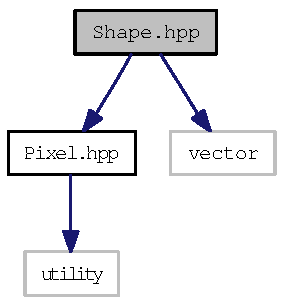
\includegraphics[width=86pt]{_shape_8hpp__incl}
\end{center}
\end{figure}


This graph shows which files directly or indirectly include this file:\nopagebreak
\begin{figure}[H]
\begin{center}
\leavevmode
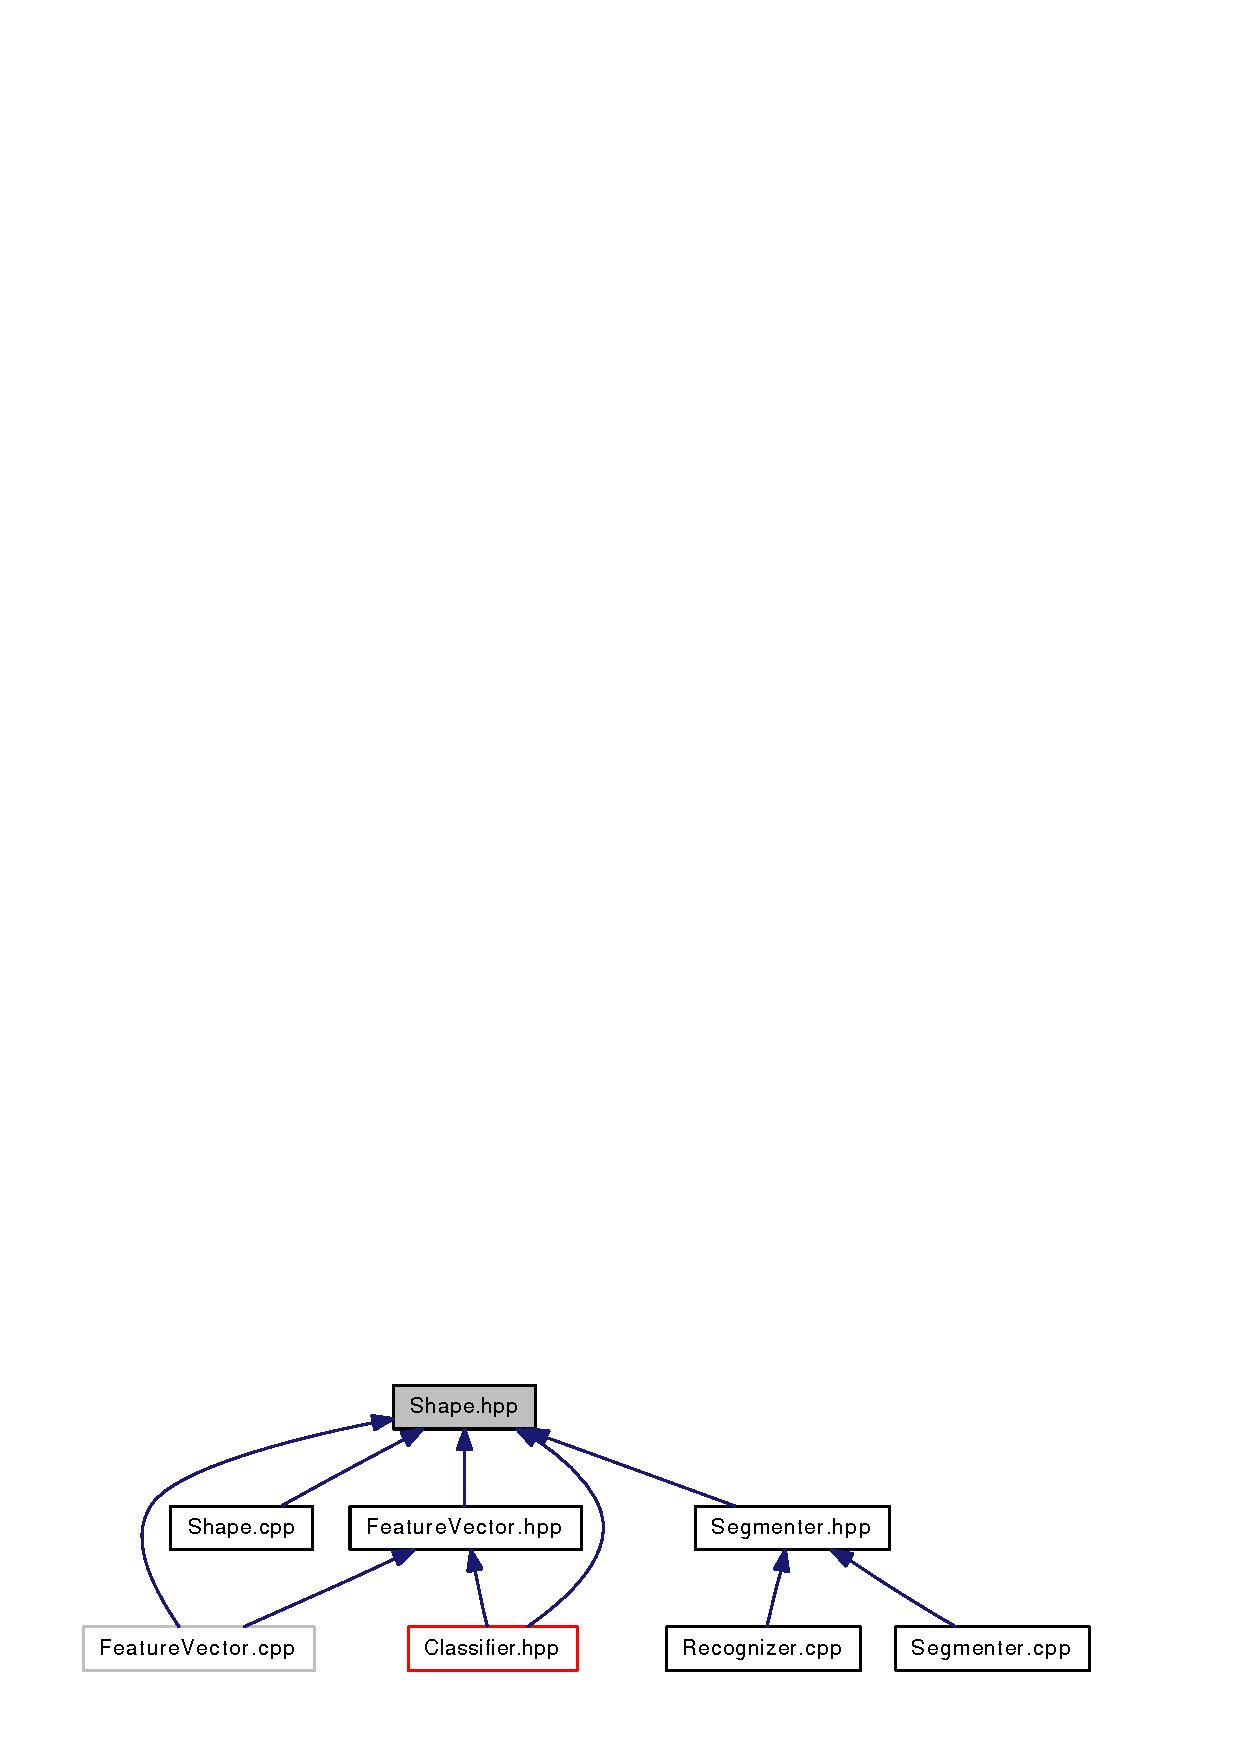
\includegraphics[width=263pt]{_shape_8hpp__dep__incl}
\end{center}
\end{figure}
\subsection*{Data Structures}
\begin{CompactItemize}
\item 
class \hyperlink{class_shape}{Shape}
\begin{CompactList}\small\item\em The shape of a character within a press clip. \item\end{CompactList}\end{CompactItemize}
